\documentclass[tikz, border=15pt]{standalone}
\usepackage{tikz}
\usetikzlibrary{arrows.meta, positioning, calc, fit, backgrounds}
\usepackage{amsmath, lmodern}
\usepackage[T1]{fontenc}

\tikzset{
  ssblock/.style = {draw, rectangle, very thick,
                    minimum width=4.0cm, minimum height=3.0cm,
                    align=center, font=\small},
  port/.style    = {draw, rectangle, thick,
                    minimum width=2.6cm, minimum height=0.55cm,
                    align=center, font=\small},
  >=Stealth, thick,
}

\begin{document}
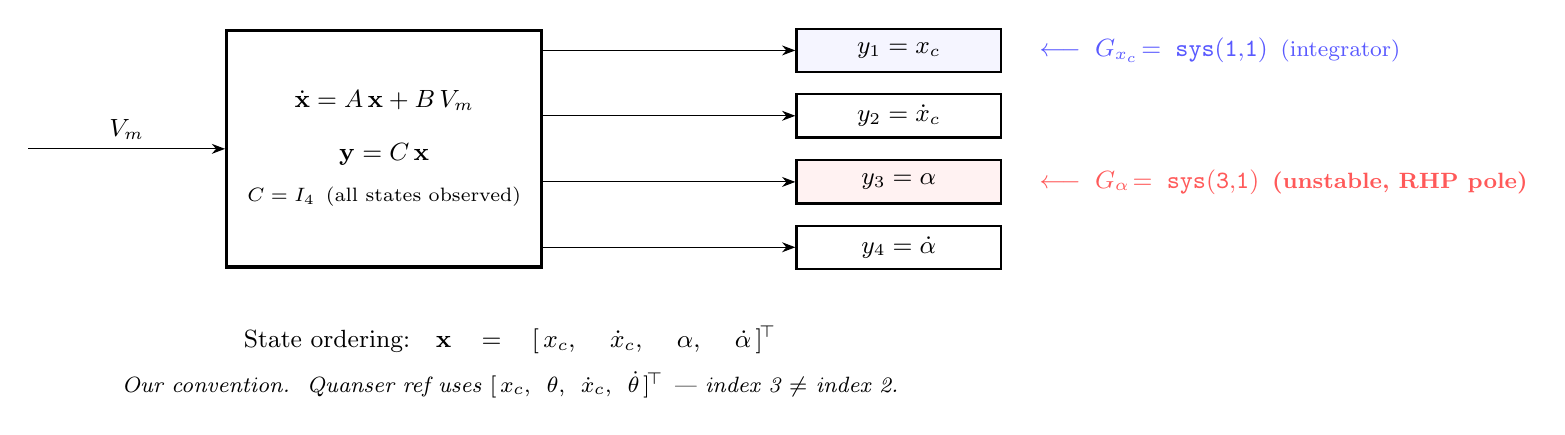
\begin{tikzpicture}

  %%──────────────────────────────────────────────────────────────────────────
  %%  STATE-SPACE BLOCK
  %%──────────────────────────────────────────────────────────────────────────
  \node[coordinate] (vin) {};

  \node[ssblock, right=2.5cm of vin] (ss)
    {$\dot{\mathbf{x}} = A\,\mathbf{x} + B\,V_m$\\[8pt]
     $\mathbf{y} = C\,\mathbf{x}$\\[4pt]
     {\scriptsize$C = I_4$\enspace(all states observed)}};

  %%──────────────────────────────────────────────────────────────────────────
  %%  OUTPUT PORTS  (one per state, stacked vertically)
  %%──────────────────────────────────────────────────────────────────────────
  \node[port, right=3.2cm of ss, yshift=+1.25cm, fill=blue!4]   (p1) {$y_1 = x_c$};
  \node[port, right=3.2cm of ss, yshift=+0.42cm]                (p2) {$y_2 = \dot{x}_c$};
  \node[port, right=3.2cm of ss, yshift=-0.42cm, fill=red!5]    (p3) {$y_3 = \alpha$};
  \node[port, right=3.2cm of ss, yshift=-1.25cm]                (p4) {$y_4 = \dot{\alpha}$};

  %%──────────────────────────────────────────────────────────────────────────
  %%  WIRES
  %%──────────────────────────────────────────────────────────────────────────
  %% Input
  \draw[->] (vin) -- node[above]{\small$V_m$} (ss);

  %% Outputs
  \draw[->] (ss.east |- p1) -- (p1);
  \draw[->] (ss.east |- p2) -- (p2);
  \draw[->] (ss.east |- p3) -- (p3);
  \draw[->] (ss.east |- p4) -- (p4);

  %%──────────────────────────────────────────────────────────────────────────
  %%  SISO PLANT EXTRACTION LABELS
  %%──────────────────────────────────────────────────────────────────────────
  \node[font=\small, blue!65, anchor=west] at ($(p1.east)+(0.35, 0)$)
    {$\longleftarrow\;G_{x_c}\!=\;\mathtt{sys(1,\!1)}$\enspace
     {\footnotesize(integrator)}};

  \node[font=\small, red!65, anchor=west] at ($(p3.east)+(0.35, 0)$)
    {$\longleftarrow\;G_{\alpha}\!=\;\mathtt{sys(3,\!1)}$\enspace
     {\footnotesize\textbf{(unstable, RHP pole)}}};

  %%──────────────────────────────────────────────────────────────────────────
  %%  STATE VECTOR ANNOTATION (below)
  %%──────────────────────────────────────────────────────────────────────────
  \node[font=\small, anchor=north, text width=11cm, align=center]
    at ($(ss.south)+(1.6cm, -0.6cm)$)
    {State ordering:\quad
     $\mathbf{x} = [\,x_c,\;\dot{x}_c,\;\alpha,\;\dot{\alpha}\,]^{\!\top}$\\[5pt]
     {\footnotesize\itshape
      Our convention.\ \
      Quanser ref uses
      $[\,x_c,\;\theta,\;\dot{x}_c,\;\dot{\theta}\,]^{\!\top}$
      --- index 3 $\neq$ index 2.}};

\end{tikzpicture}
\end{document}
